% !TEX program = xelatex
% !TEX program = xelatex

\documentclass[hidelinks, 12pt, a4paper]{article}

\usepackage{fontspec}
\setmainfont[Ligatures=TeX]{Linux Libertine O}

\usepackage[hidelinks, colorlinks = true, urlcolor = blue]{hyperref}

\usepackage{indentfirst}
\usepackage{graphicx}
\usepackage[left=2cm,right=2cm,top=2cm,bottom=2cm]{geometry}
\usepackage{lipsum}


\begin{document}

\begin{titlepage}

\begin{figure}[h!]
  \begin{center}
    
\includegraphics[width=3cm]{assets/auth.pdf}
    \label{fig:cover_auth_logo}
  \end{center}
\end{figure}

\centering
\Large Αριστοτέλειο Πανεπιστήμιο Θεσσαλονίκης\\
\Large Πολυτεχνική Σχολή\\
%\large Τμήμα Ηλεκτρολόγων Μηχανικών και Μηχανικών Υπολογιστών\\
%\large Τομέας Τηλεπικοινωνιών

\vspace{\fill}

\LARGE \textbf{Java socket programming} \\
\LARGE \textbf{Δίκτυα 2}

\vspace{\fill}

\Large Θεόδωρος Κατζάλης \\
\Large ΑΕΜ:9282 \\ 
\Large katzalis@auth.gr

\vspace{\fill}
\raggedright

\centering
\vspace{\fill}
\today

\end{titlepage}

%\maketitle


\pagebreak
\tableofcontents
\pagebreak

% \section{Lorem}
% \lipsum


\section{G1}

Info:
The request code is E0818 
Tic: 2020-11-29T14:35:34.271520
Toc: 2020-11-29T14:39:35.015592

\begin{figure}[h!]
\centering
	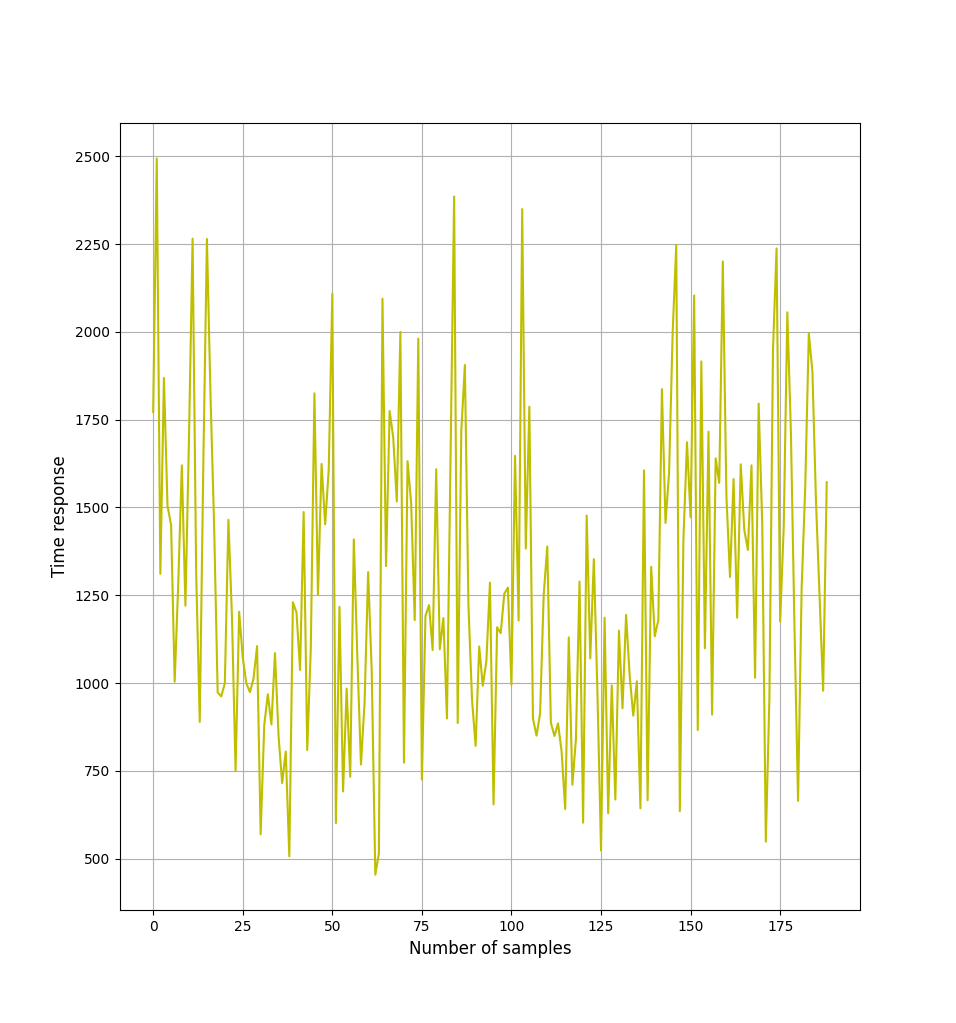
\includegraphics[height=.38\textheight, width=\textwidth]{assets/session2/g1.png}
	\caption{G1} 
\end{figure}

\section{G2}

\begin{figure}[h!]
\centering
	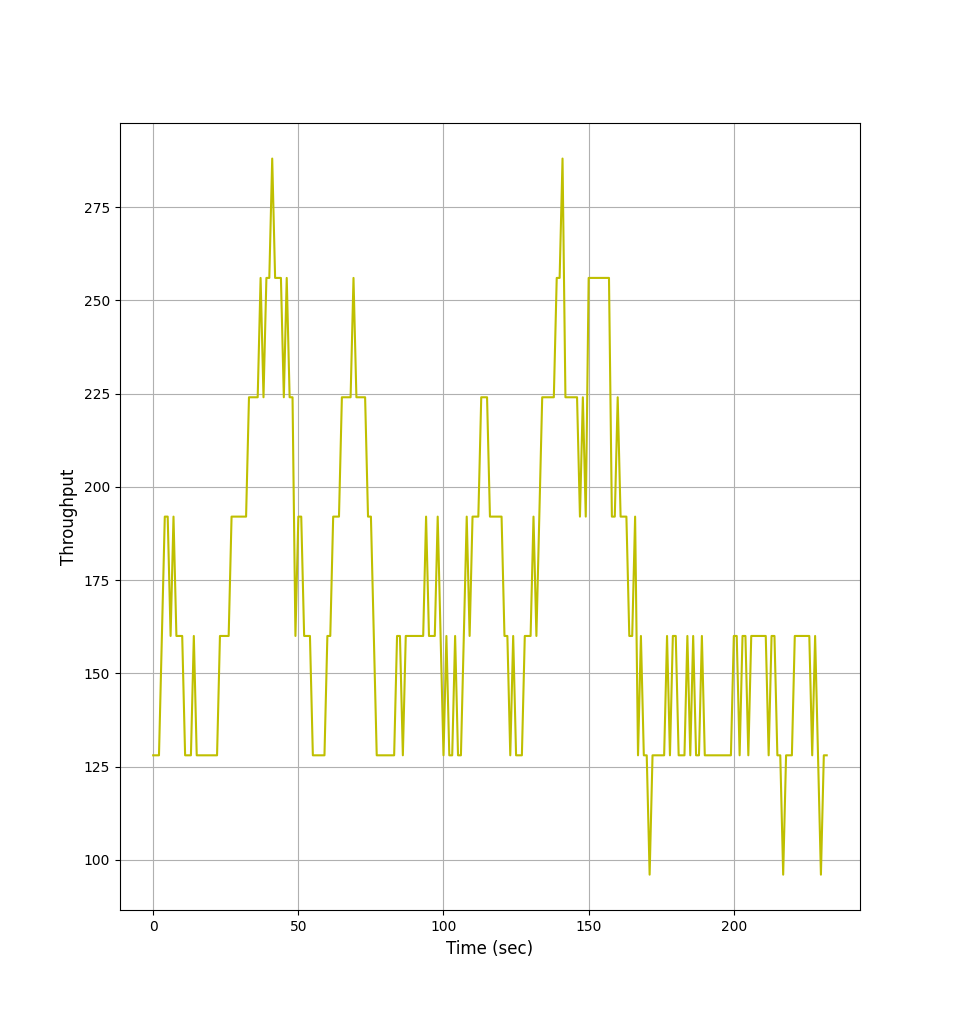
\includegraphics[height=.38\textheight, width=\textwidth]{assets/session2/g2.png}
	\caption{G2} 
\end{figure}

%\pagebreak

\section{G3}

\begin{figure}[h!]
\centering
	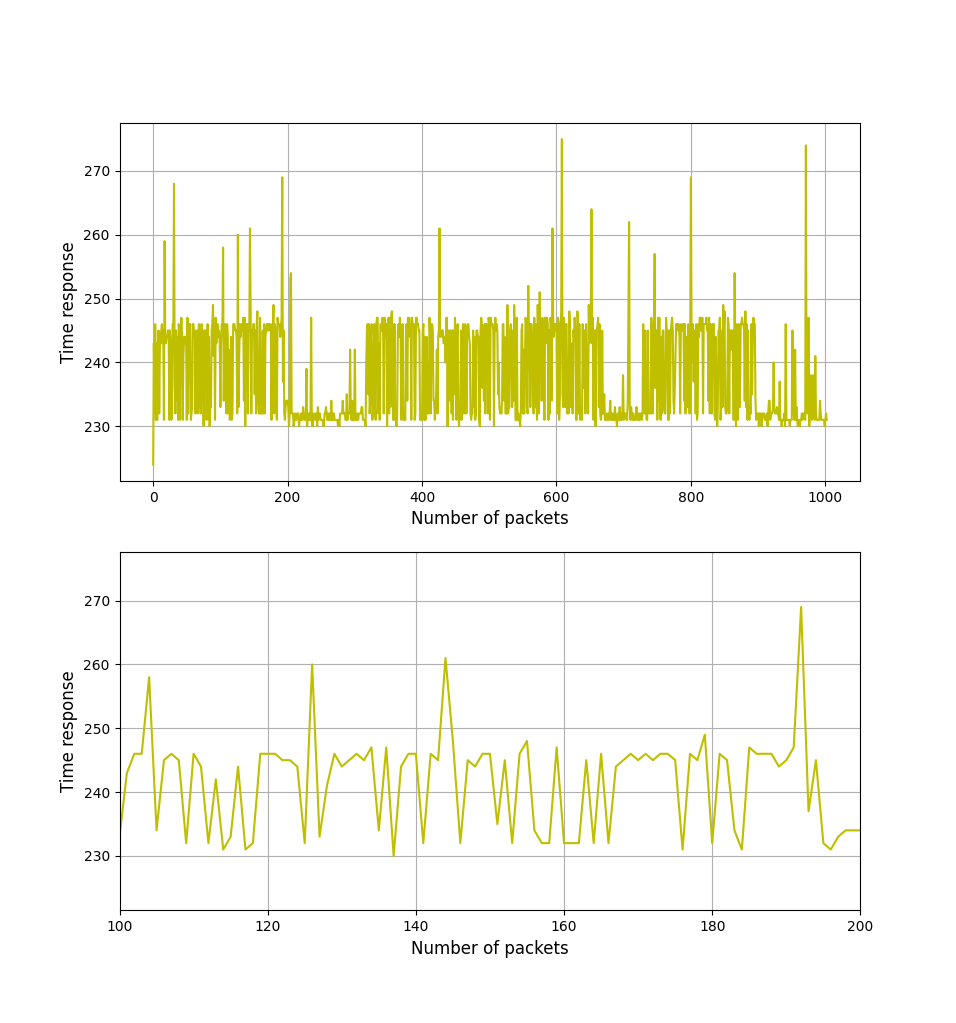
\includegraphics[height=.38\textheight, width=\textwidth]{assets/session2/g3.png}
    \caption{G3. Zoom in (below figure)} 
\end{figure}

\section{G4}

\begin{figure}[h!]
\centering
	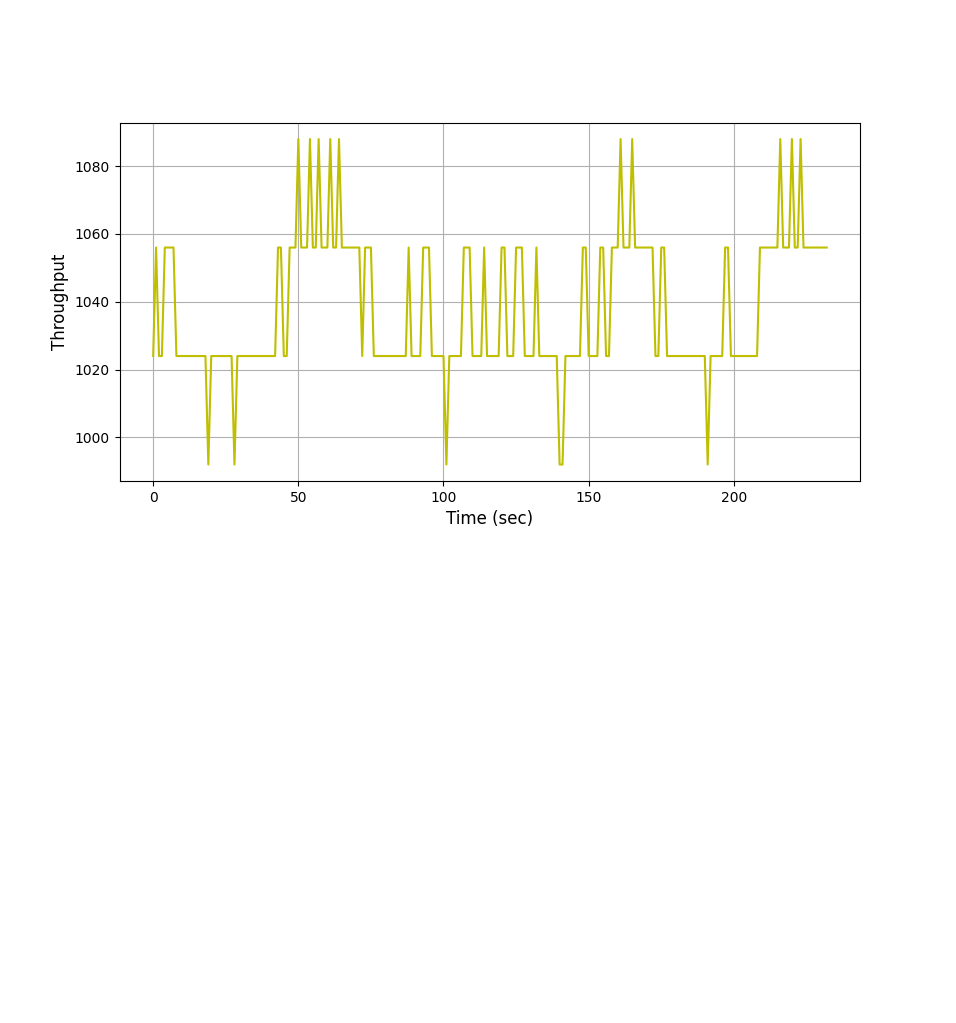
\includegraphics[height=.38\textheight, width=\textwidth]{assets/session2/g4.png}
	\caption{G4} 
\end{figure}

\section{G5}

\begin{figure}[h!]
	\centering
		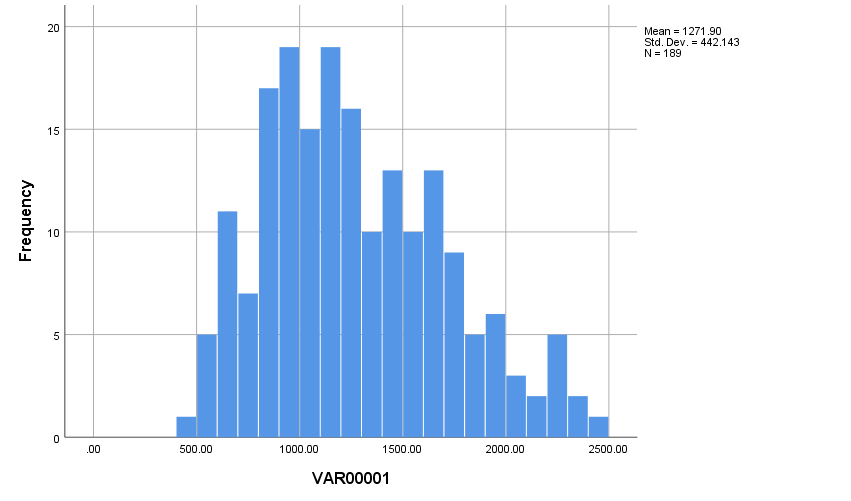
\includegraphics[height=.38\textheight, width=\textwidth]{assets/session2/g5.png}
		\caption{G5 histogram samples with delay} 
	\end{figure}

\section{G6}

\begin{figure}[h!]
	\centering
		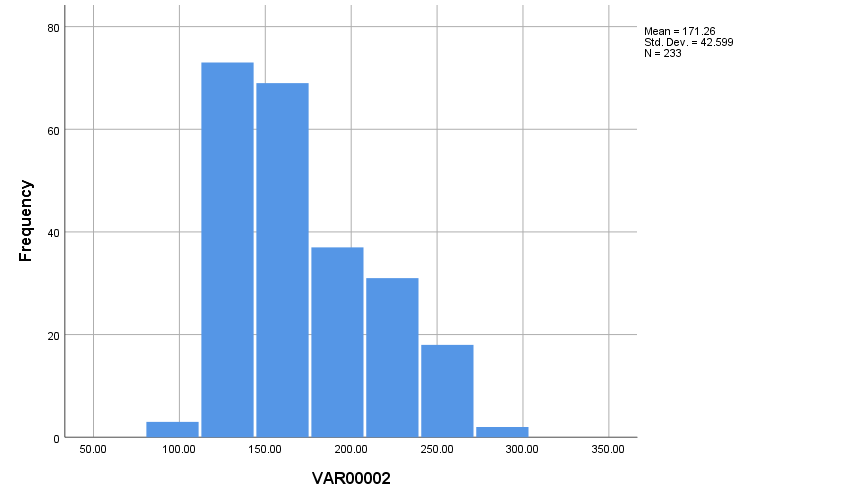
\includegraphics[height=.38\textheight, width=\textwidth]{assets/session2/g6.png}
		\caption{G5 histogram throughput with delay} 
	\end{figure}

\section{G7}

\begin{figure}[h!]
	\centering
		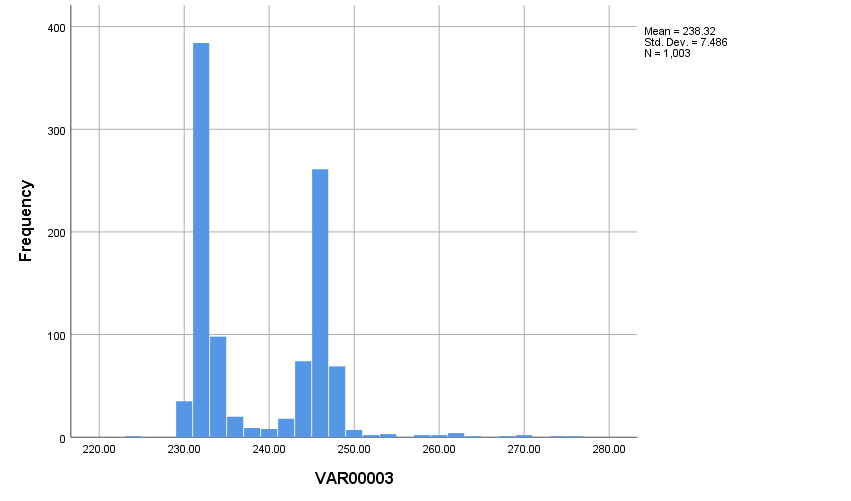
\includegraphics[height=.38\textheight, width=\textwidth]{assets/session2/g7.png}
		\caption{G5 histogram samples with no delay} 
	\end{figure}

\section{G8}

\begin{figure}[h!]
	\centering
		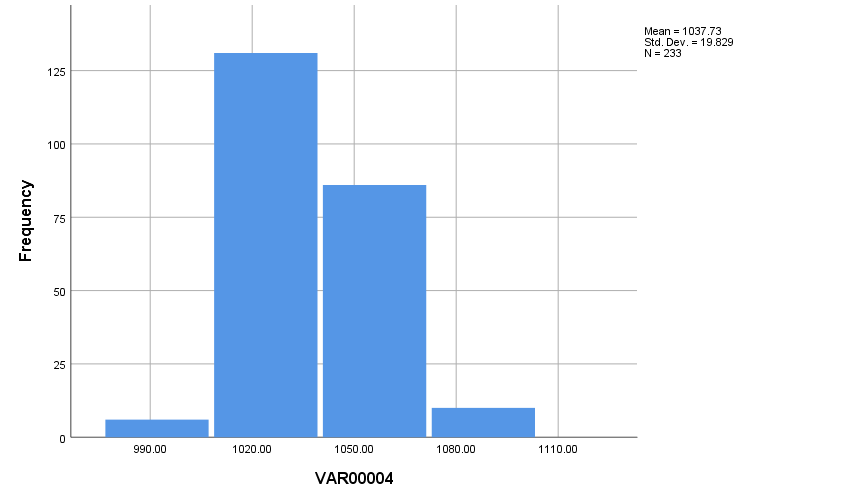
\includegraphics[height=.38\textheight, width=\textwidth]{assets/session2/g8.png}
		\caption{G5 histogram throughput with no delay} 
	\end{figure}

\section{R1}


Εσκεμμένα αφήσαμε το ίδο Κ = 1.8, προκειμένου να δείξουμε οτι ανάλογα τις συνθήκες, το rto μπορεί να μην είναι το βέλτιστο, όπως και στην προκειμένη περίπτωση όπου υπάρχουν κάποια σημεία όπου το rtt είναι υψηλότερα απο το rto, το οποίο δηλώνει ότι θα διακόπταμε την επικοινωνία προτού εξαληφθούν όλες οι πιθανότητες λήψης πακέτου.

\begin{figure}[h!]
\centering
	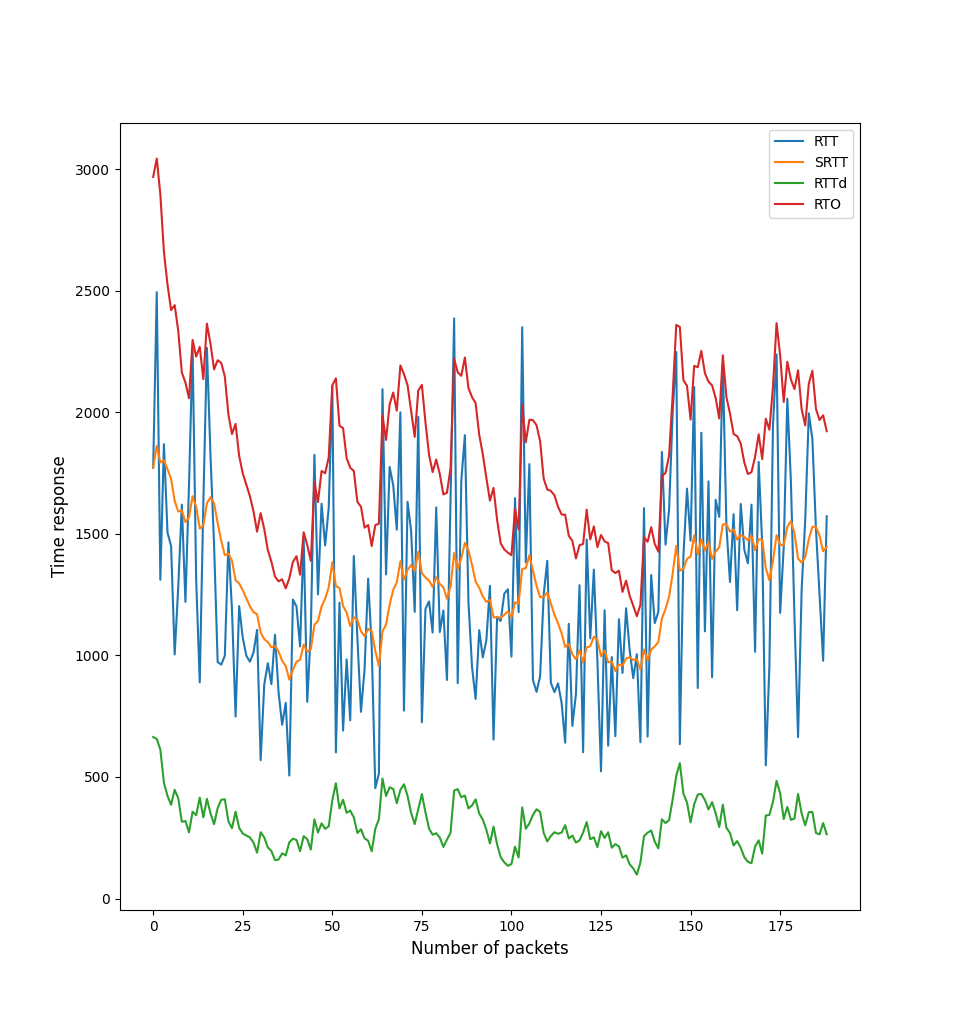
\includegraphics[height=.38\textheight, width=\textwidth]{assets/session2/r1.png}
	\caption{Retransmission timeout} 
\end{figure}



\section{E1}

\begin{figure}[h!]
\centering
	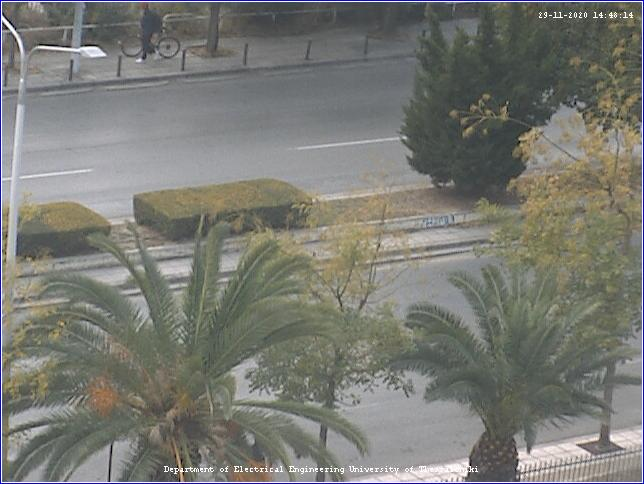
\includegraphics[height=.38\textheight, width=\textwidth]{assets/session2/image_fix.jpg}
	\caption{E1} 
\end{figure}
CAM=FIX
M2685UDP=1024
2020-11-29T14:48:14.330279
2020-11-29T14:48:20.694735


\section{E2}

\begin{figure}[h!]
\centering
	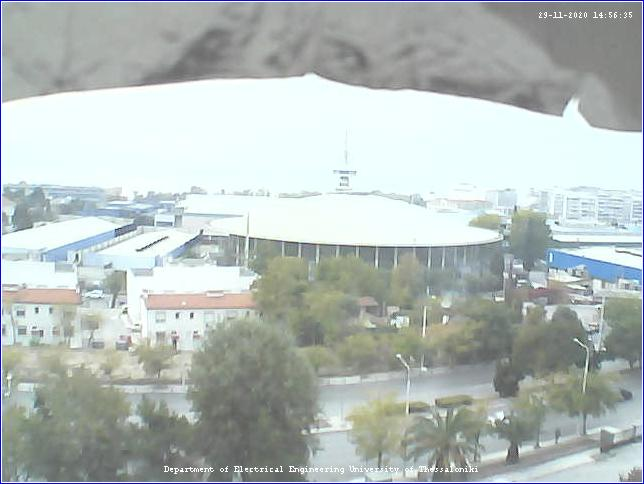
\includegraphics[height=.38\textheight, width=\textwidth]{assets/session2/image_ptz.jpg}
	\caption{E2 Image code:M5983CAM=PTZ} 
\end{figure}
CAM=PTZDIR=R
M2685UDP=1024
2020-11-29T14:59:24.061992
2020-11-29T14:59:31.174414


\section{Temperature}

\begin{figure}[h!]
\centering
	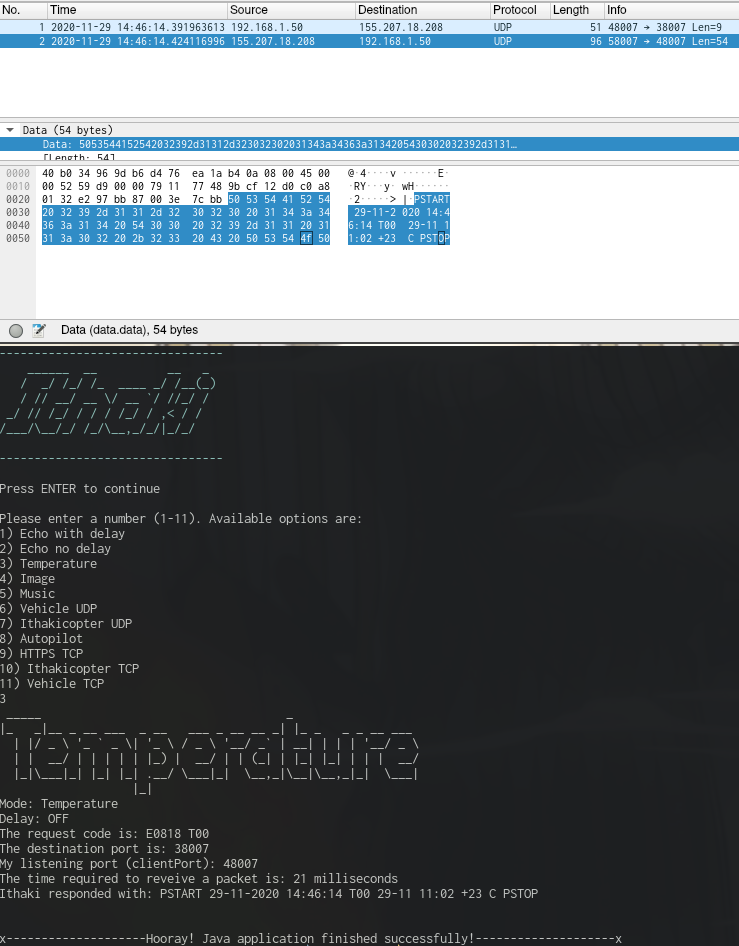
\includegraphics[height=.38\textheight, width=.8\textwidth]{assets/session2/temp.png}
	\caption{Temperature} 
\end{figure}
Info Temperature app:
E0818 
2020-11-29T14:46:14.374502
2020-11-29T14:46:14.428539


\section{G9}

\begin{figure}[h!]
\centering
	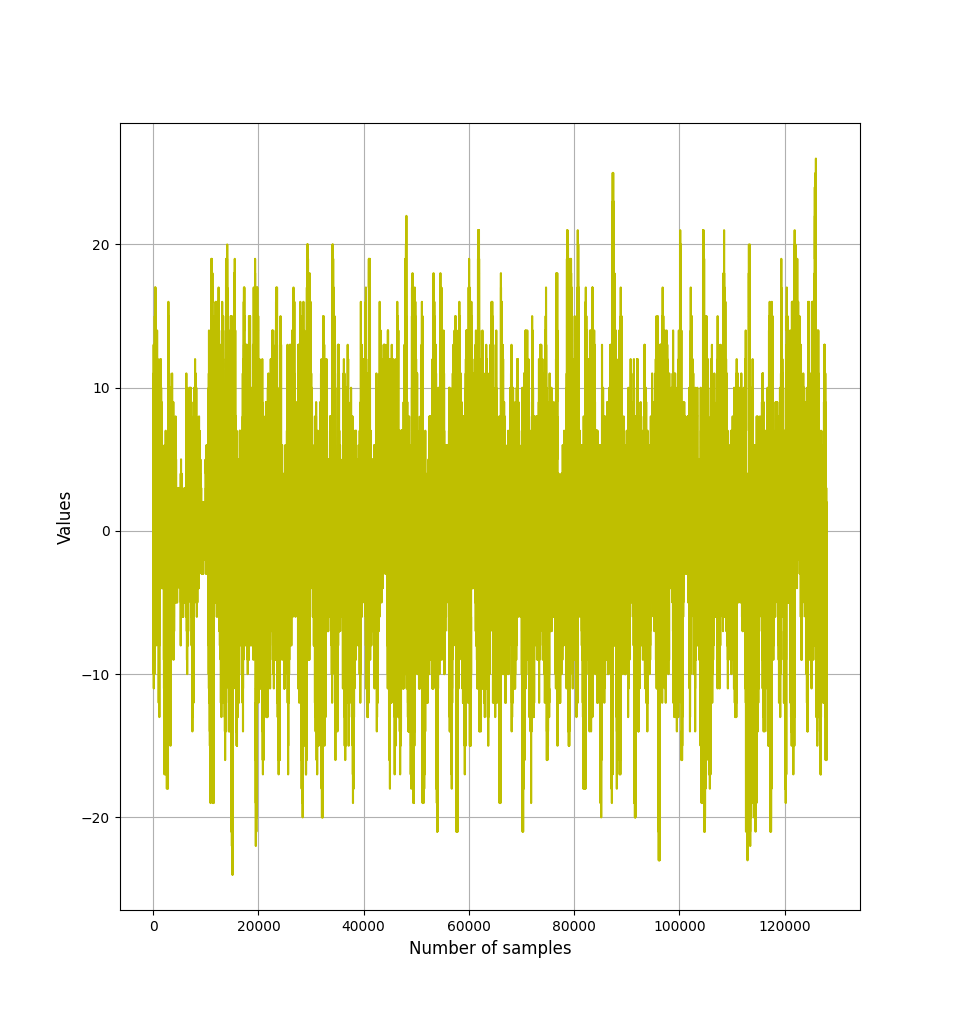
\includegraphics[height=.38\textheight, width=\textwidth]{assets/session2/g9.png}
	\caption{G9 DPCM samples waveform L01} 
\end{figure}
A1631
Encoding: 
Type: F2020-11-29T15:11:27.391189
2020-11-29T15:12:02.977637

\section{G10}

\begin{figure}[h!]
\centering
	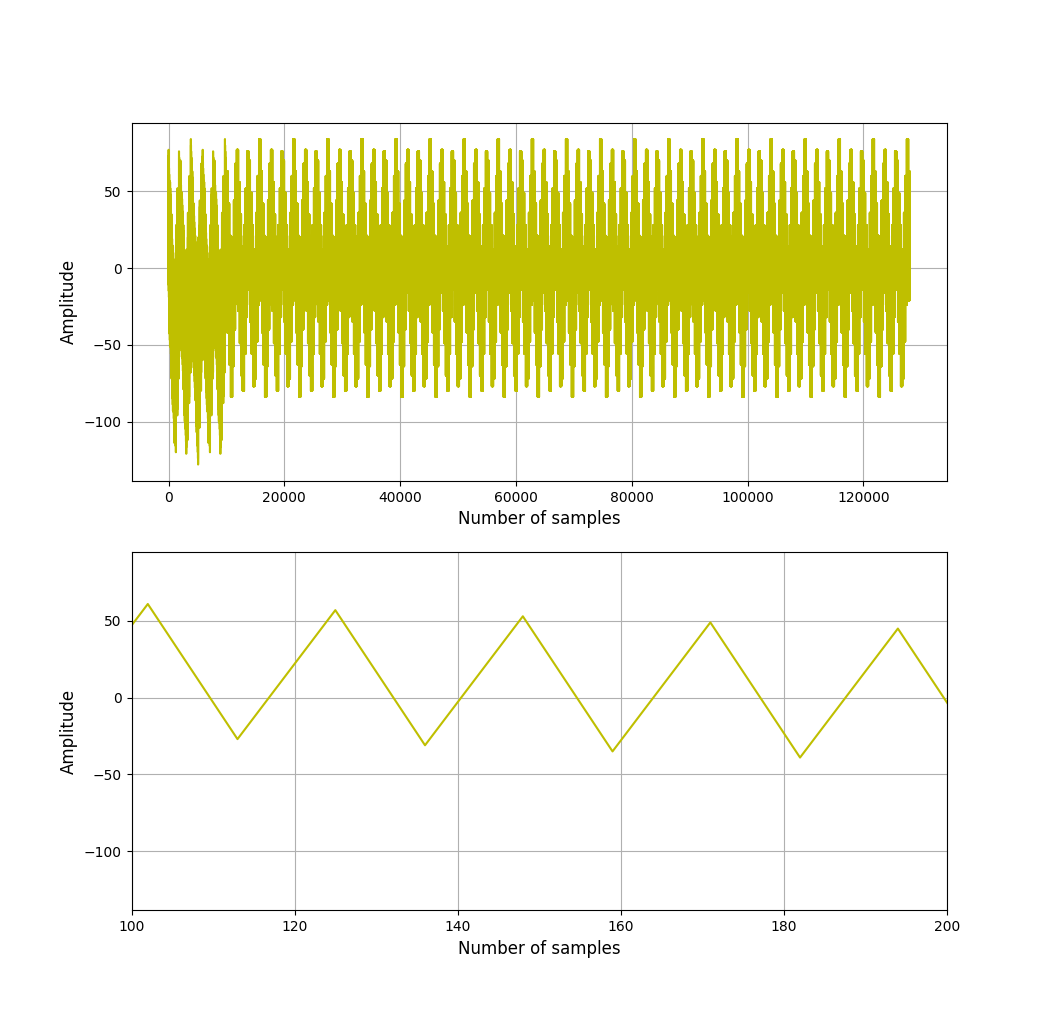
\includegraphics[height=.38\textheight, width=\textwidth]{assets/session2/g10.png}
    \caption{G10 DPCM samples waveform Tone}
\end{figure}
A1631
Encoding: 
Type: T2020-11-29T15:04:48.197746
2020-11-29T15:05:23.743341


\section{G11}

A1631
Encoding: AQ L01
Type: F2020-11-29T15:13:23.876058
2020-11-29T15:13:59.386860
\begin{figure}[h!]
\centering
	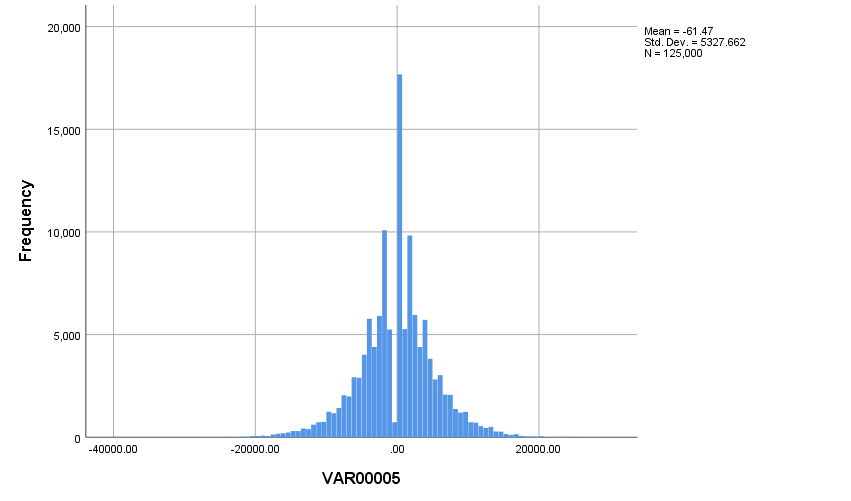
\includegraphics[height=.38\textheight, width=\textwidth]{assets/session2/g11.png}
    \caption{G11 AQDPCM diff samples}
\end{figure}

\section{G12}

\begin{figure}[h!]
	\centering
		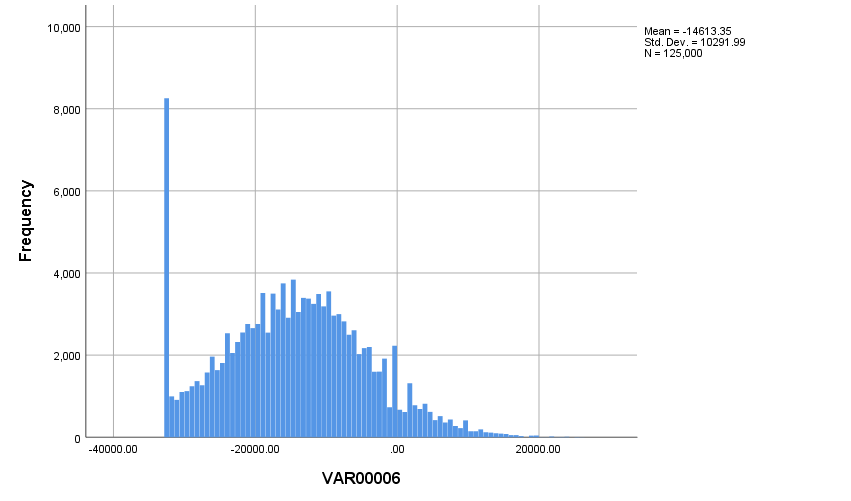
\includegraphics[height=.38\textheight, width=\textwidth]{assets/session2/g12.png}
		\caption{G12 AQDPCM  samples}
	\end{figure}

\section{G13}
A1631
Encoding: 
Type: F2020-11-29T15:11:27.391189
2020-11-29T15:12:02.977637
\begin{figure}[h!]
	\centering
		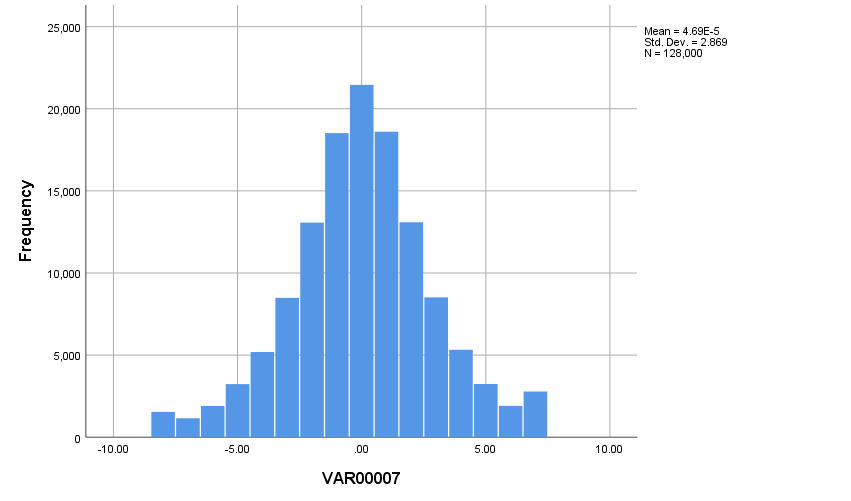
\includegraphics[height=.38\textheight, width=\textwidth]{assets/session2/g13.png}
		\caption{G13 DPCM diff samples}
	\end{figure}

\section{G14}
\begin{figure}[h!]
	\centering
		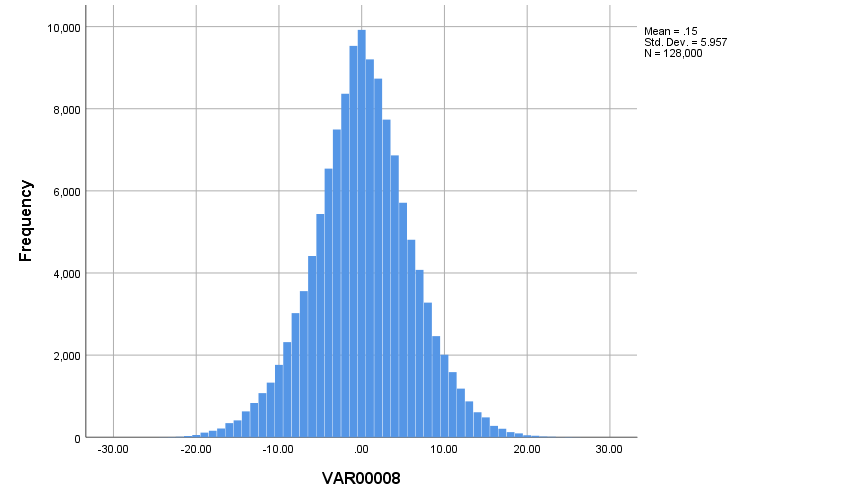
\includegraphics[height=.38\textheight, width=\textwidth]{assets/session2/g14.png}
		\caption{G14 DPCM  samples}
	\end{figure}

\section{G15}
A1631
Encoding: AQ L01
Type: F2020-11-29T15:13:23.876058
2020-11-29T15:13:59.386860
\begin{figure}[h!]
\centering
	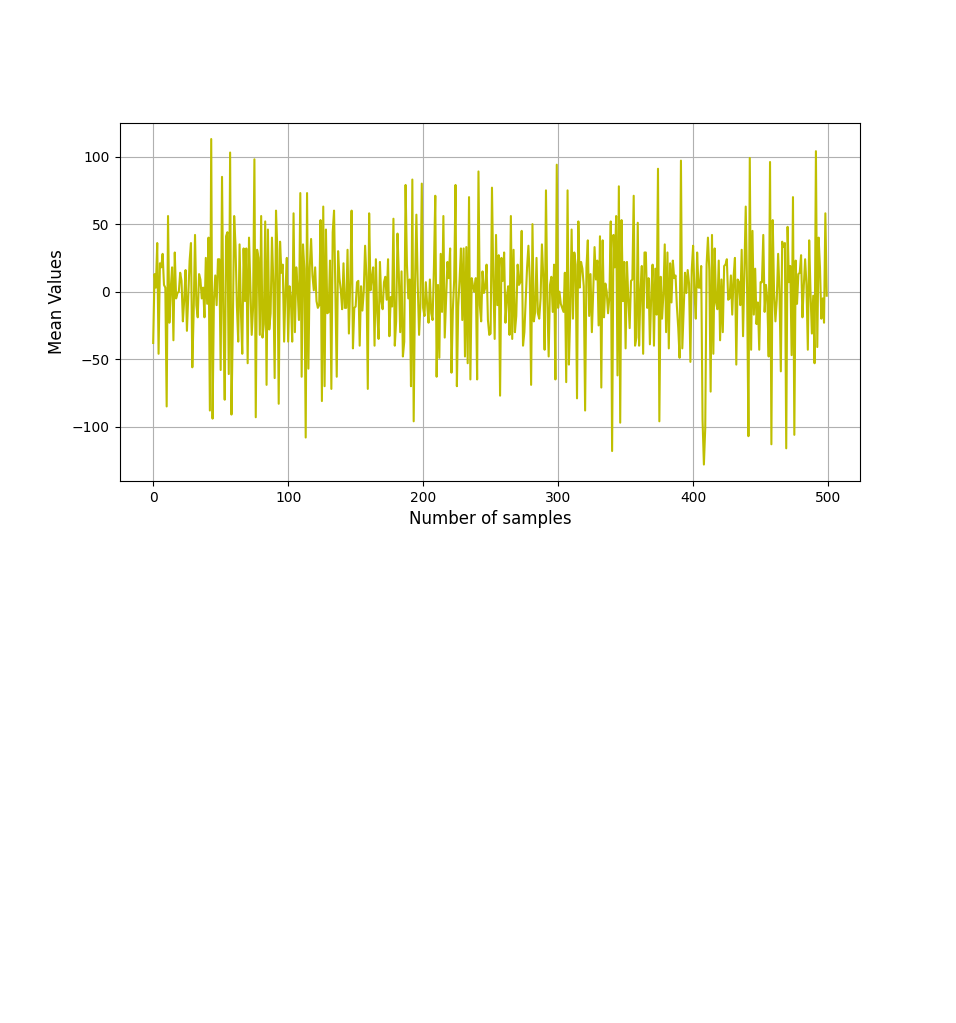
\includegraphics[height=.38\textheight, width=\textwidth]{assets/session2/g15.png}
    \caption{G15 Mean 1st clip}
\end{figure}

\section{G16}

\begin{figure}[h!]
\centering
	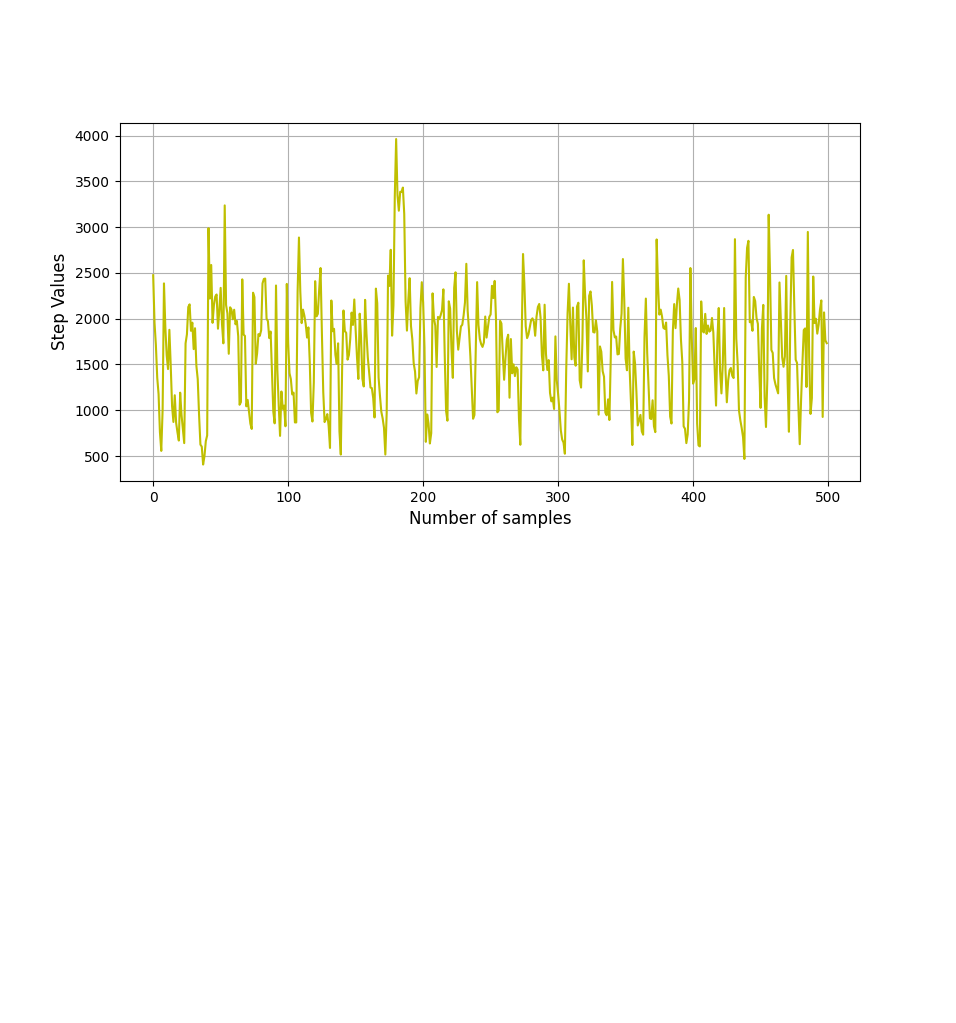
\includegraphics[height=.38\textheight, width=\textwidth]{assets/session2/g16.png}
    \caption{G16 Step 1st clip  }
\end{figure}

\section{G17}
A1631
Encoding: AQ
Type: F2020-11-29T15:15:41.614991
2020-11-29T15:16:17.079048
L02
\begin{figure}[h!]
\centering
	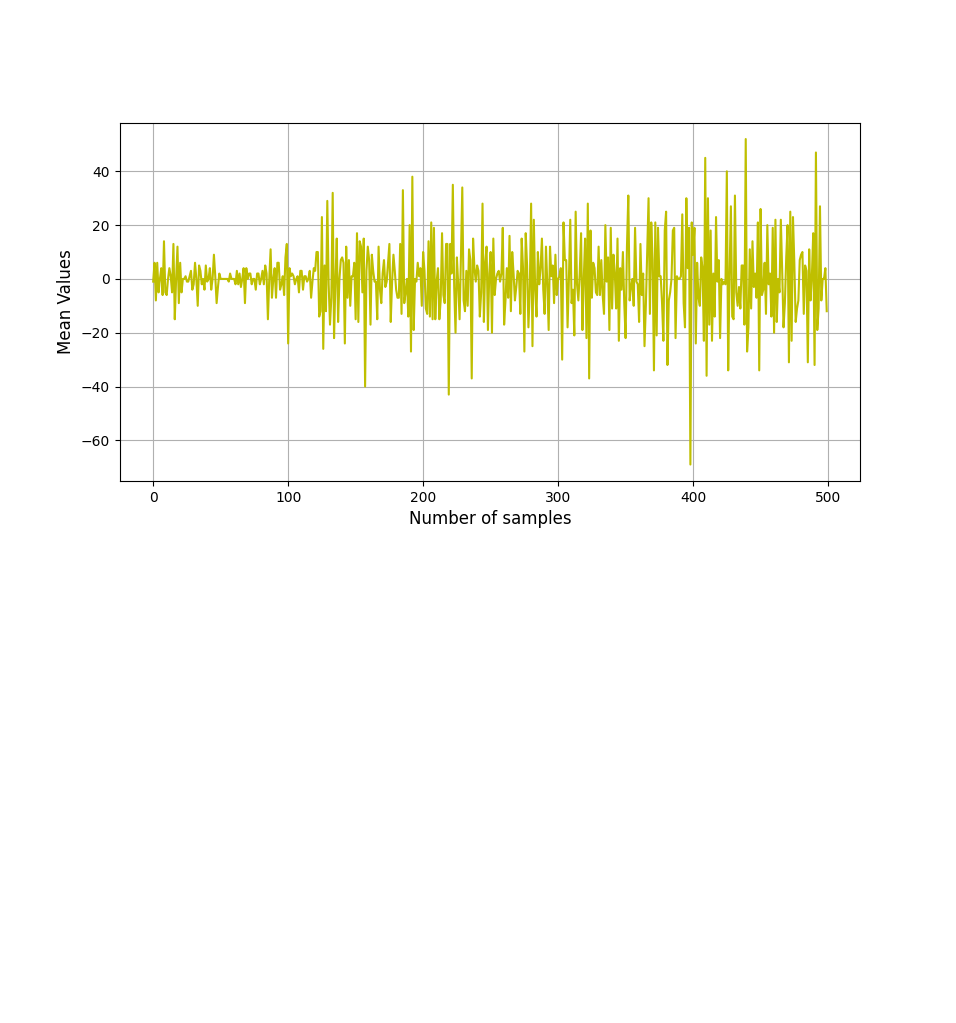
\includegraphics[height=.38\textheight, width=\textwidth]{assets/session2/g17.png}
    \caption{G17 Mean 2nd clip}
\end{figure}



\section{G18}

\begin{figure}[h!]
\centering
	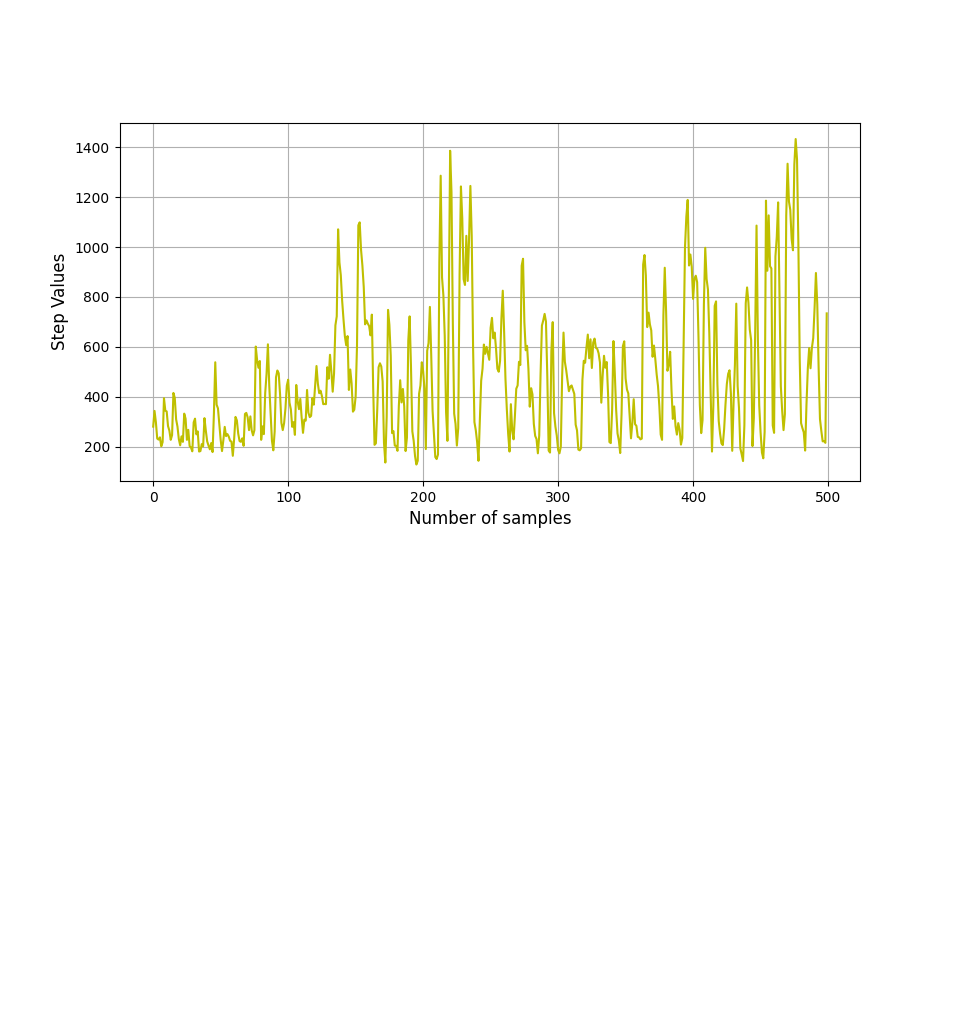
\includegraphics[height=.38\textheight, width=\textwidth]{assets/session2/g18.png}
    \caption{G18 Step 2nd clip}
\end{figure}



\section{G19}
Πρώτη μέτρηση
Info Ithakicopter app:
2020-11-29T15:25:31.439784
2020-11-29T15:27:02.330775

\begin{figure}[h!]
\centering
	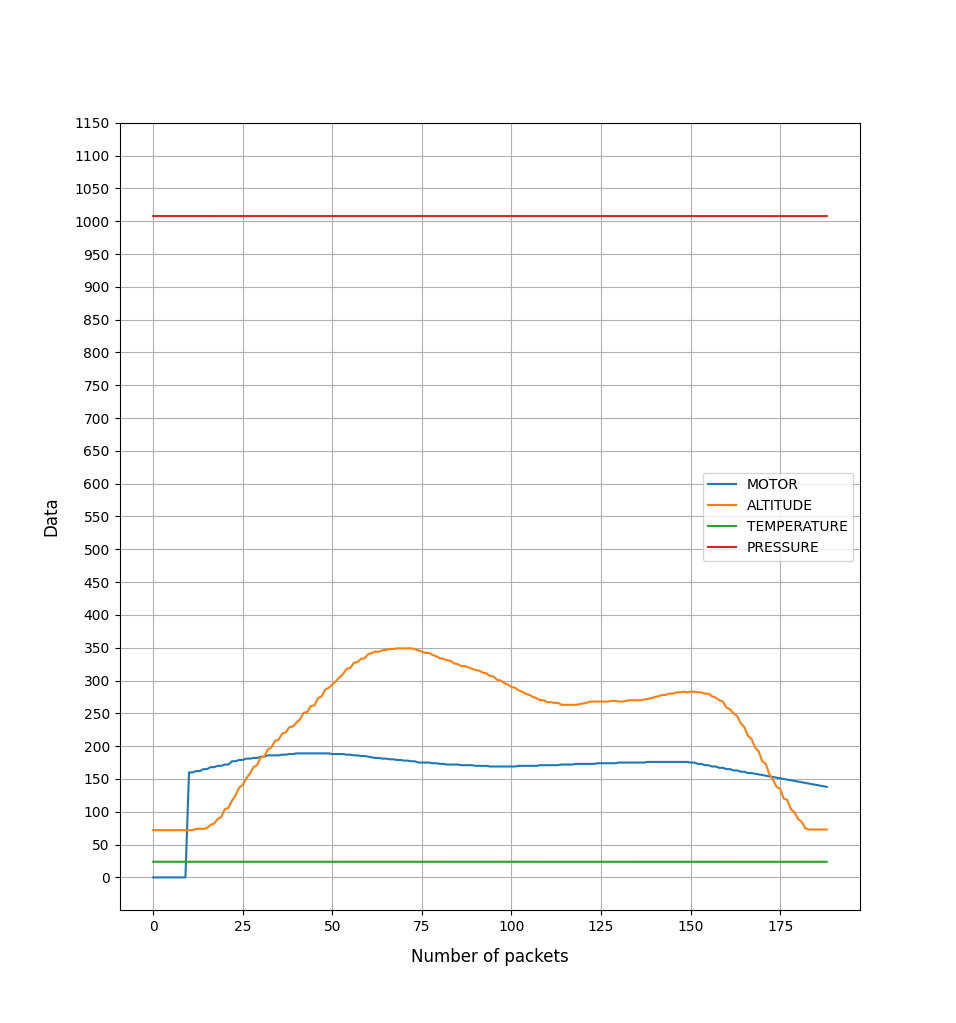
\includegraphics[height=.4\textheight, width=\textwidth]{assets/session2/g19.png}
    \caption{G19 Flightlevel περίπου 280}
\end{figure}

\section{G20}

\begin{figure}[h!]
\centering
	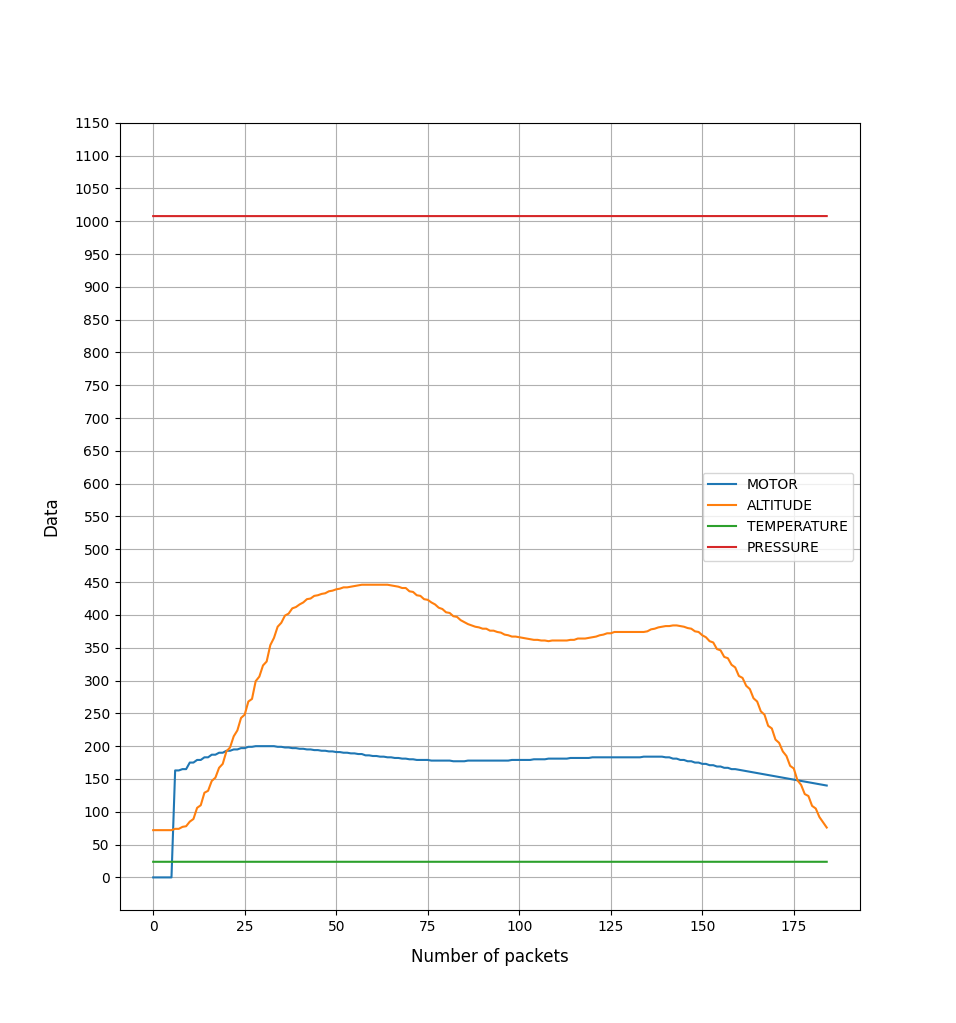
\includegraphics[height=.4\textheight, width=\textwidth]{assets/session2/g20.png}
    \caption{G20 Flightlevel περίπου 400}
\end{figure}

Info Ithakicopter app:
2020-11-29T15:27:23.485265
2020-11-29T15:28:53.387477

\section{G21}
Info Vehicle app:
2020-11-29T15:17:58.434735
2020-11-29T15:21:59.014642

\begin{figure}[h!]
\centering
	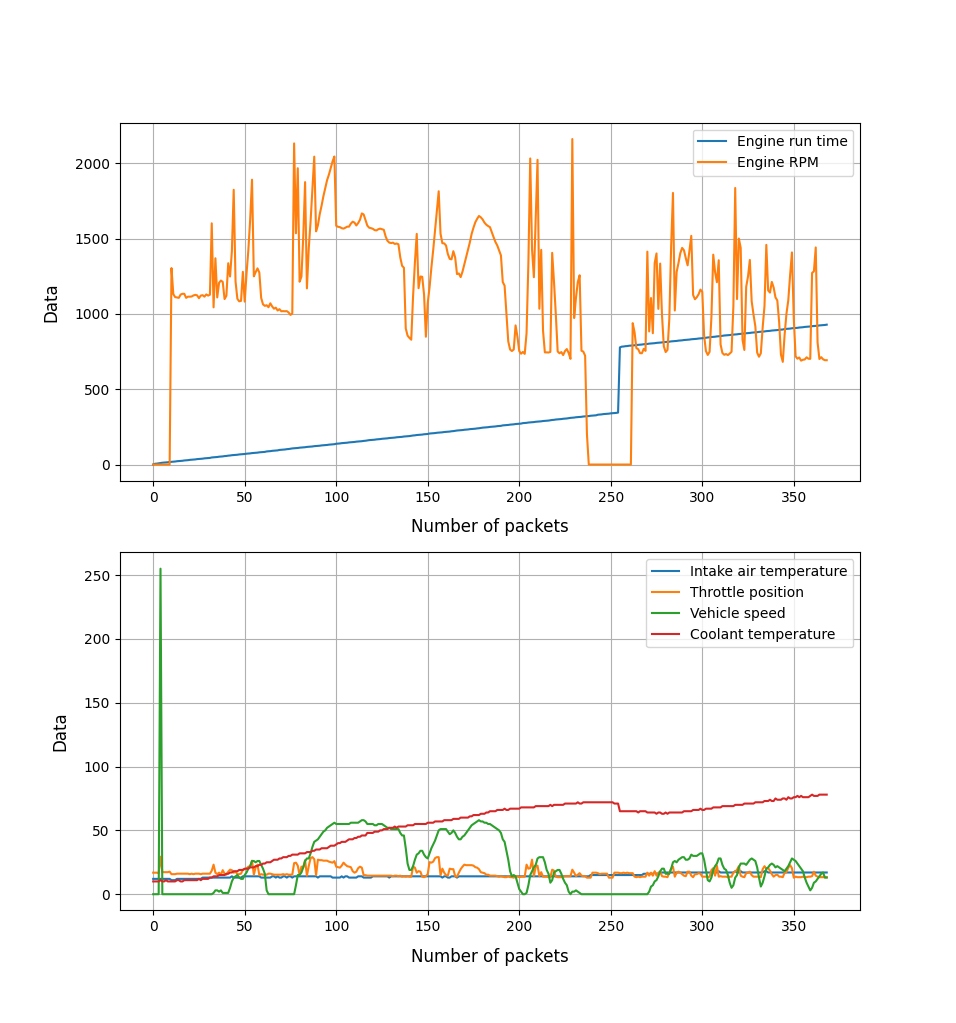
\includegraphics[height=.5\textheight, width=\textwidth]{assets/session2/g21.png}
    \caption{G21 Vehicle OBD}
\end{figure}

\end{document}
